\section{Introduction}
\label{sec:introduction}

\subsection{Why the question matters}

Knowledge graphs store facts as typed links between entities. In biomedicine,
PrimeKG links drugs, diseases and proteins \cite{chandak2023primekg}. Such a
graph is used by following short paths. Drug-repurposing methods score a drug
for a disease by the proteins the two share, or by how close the drug's targets
lie to the disease proteins in the interaction network
\cite{guney2016network}. Retrieval-augmented language models answer questions
from the neighborhood of a few hops around the entities in the question
\cite{edge2024graphrag}. In both uses, a fact is useful only if a short path to
it survives.

Real knowledge graphs lose links all the time, through incomplete curation,
retracted findings, or a data source that drops out of a merge. Their health is
usually judged with global statistics, chief among them the size of the giant
component. This is the quantity that network robustness studies track under
random failure and targeted attack \cite{albert2000error,callaway2000network}.
We ask whether that statistic tells us anything about the short paths that
applications actually use.

\subsection{The answer in one figure}

Figure~\ref{fig:summary} answers the question on a 5,000-node sample of PrimeKG
and a fixed benchmark of 200 drug--disease queries. Each query asks whether a
drug and a disease are still linked through a shared protein within $L$ hops.
Panel~(a) removes edges at random. With half of the edges gone, 98\% of nodes
are still in the giant component and 86\% of queries can still be reached by a
path of any length, but only 41\% keep a two-hop answer. Panel~(b) removes 5\%
of nodes, either at random or by targeting the highest-degree or
highest-betweenness nodes. The attacks cost the giant component 6--7
percentage points more than random removal, but they cost two-hop retrieval
57--63 points more. The giant component therefore misses most of the functional
damage, and it understates the extra harm of targeted damage by nearly an order
of magnitude.

\begin{figure}[!htbp]
  \centering
  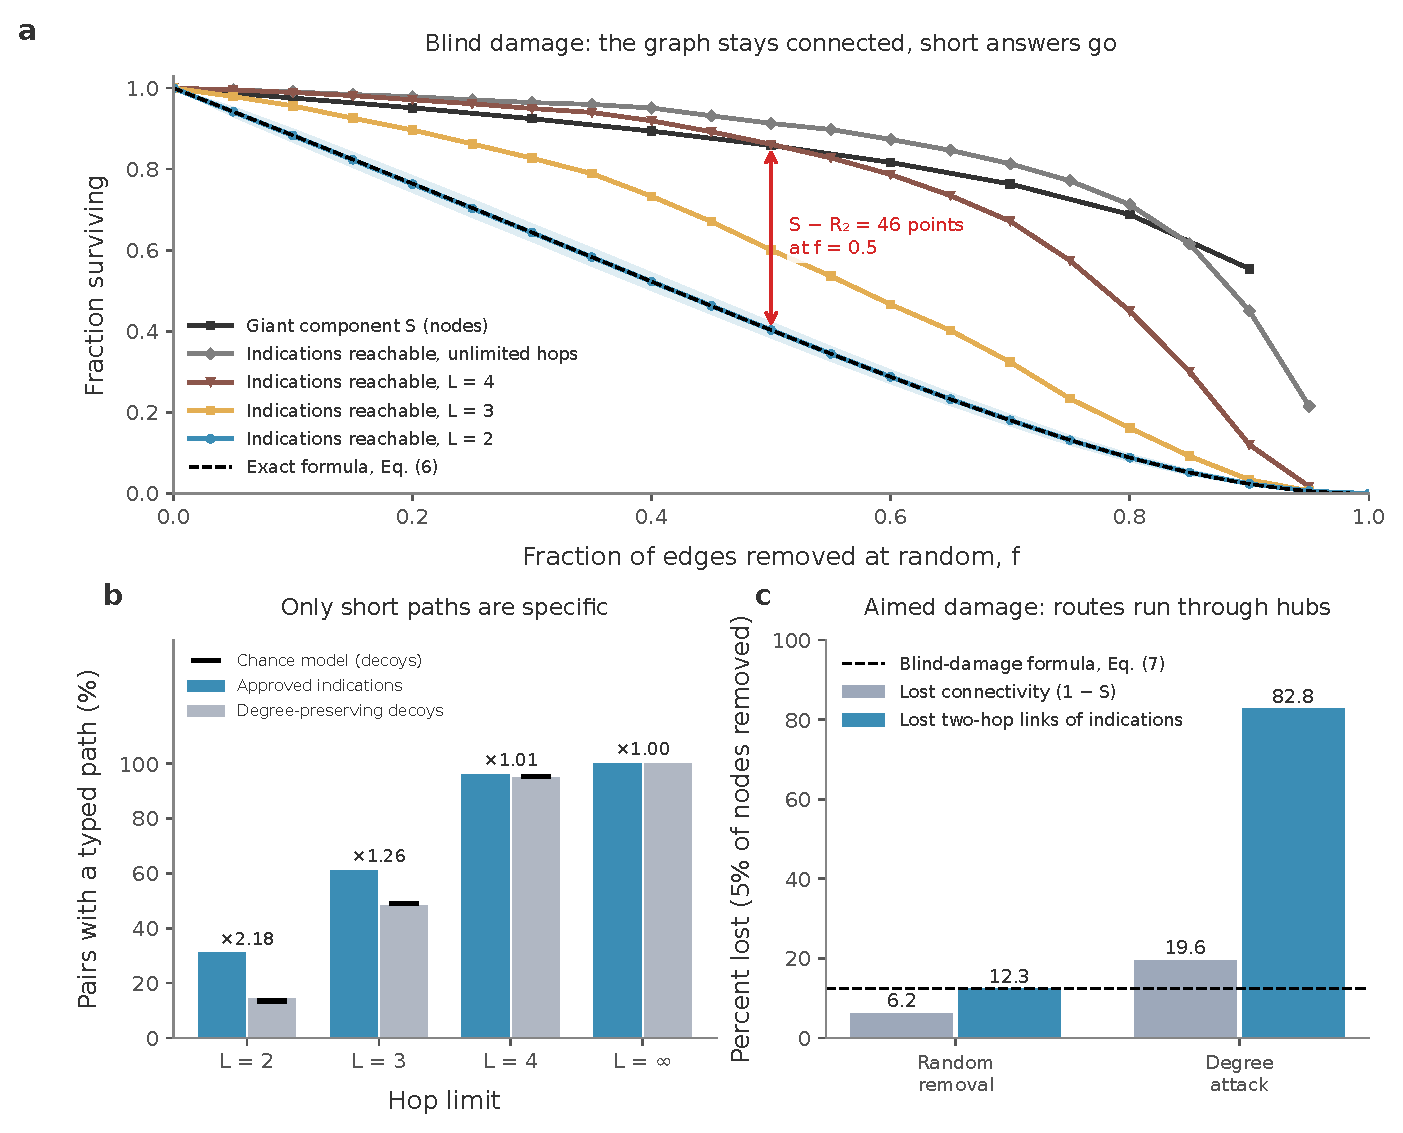
\includegraphics[width=\linewidth]{act0/fig_summary.pdf}
  \caption{The main results. (a) Random edge removal: giant component $S$
  (mean of ten damage orders) and retrieval success $R_L$ with hop limit $L$
  (mean of 600 independent damage orders). Shading shows the spread of a single
  damage state (one standard deviation). Dashed lines are the predictions of
  Section~\ref{sec:theory}, which contain no fitted parameters. (b) Damage after
  removing 5\% of nodes at random (mean of ten orders) or by a fixed degree or
  betweenness ranking. The dashed line shows the two-hop loss expected if the
  same number of nodes were removed blindly.}
  \label{fig:summary}
\end{figure}

\subsection{What explains it}

The course treated connectivity with generating functions and percolation. We
show that one simple principle covers connectivity and retrieval together. A
quantity survives damage if at least one of its redundant units survives, so
its survival probability is one minus the generating function of its redundancy
distribution, evaluated at the failure probability of one unit
(Section~\ref{sec:theory}). The three curves in Figure~\ref{fig:summary}a
differ because they use different units and different redundancy
distributions:
\begin{itemize}[leftmargin=*,itemsep=1pt]
\item nodes have a median of 25 edges, and only 2\% have a single edge;
\item the median query has a minimum cut of 6 edges between its drug and its
disease, and 22\% have a cut of one;
\item half of the queries have exactly one shared protein.
\end{itemize}
The principle is exact for two-hop retrieval under blind damage and
approximate for the other two. It also makes clear where it must fail: when
damage is aimed at hubs, because many of the redundant units of a query sit on
hubs.
Most of the gap between $S$ and $R_2$ is due to the hop limit, not to
fragmentation of the graph.

\subsection{Contributions}

\begin{enumerate}[leftmargin=*,itemsep=2pt]
\item \textbf{A common description.} We describe connectivity, unlimited-hop
reachability and bounded-hop retrieval as the same expression with three
different redundancy distributions. We separate what is exact from what is
approximate, and we test every approximation against independent simulations.
\item \textbf{An explanation of the gap.} At 50\% edge loss, needing both
endpoints to stay attached costs 12 points, and the two-hop limit costs a
further 45. Longer horizons move the bottleneck from shared proteins to drug
target links.
\item \textbf{An account of targeted damage.} Attacks violate the assumption
that every unit survives with the same probability. A degree-resolved version of
the formula reproduces the attacked retrieval rate, and we split the loss into
lost endpoints and lost routes. We use degree-preserving null models to attribute the excess structural
fragility, and we check the result on the full filtered graph.
\item \textbf{A consequence for repair.} The two-hop formula predicts the gains
of random and relation-type repair without fitting. Through the relation
types that two-hop routes use, it also explains why restoring drug and disease
links is the best policy we tested for two-hop retrieval at large budgets.
\end{enumerate}

\subsection{Beyond the course}

Lectures 6--9 developed percolation on random graphs and on interdependent
networks. Four ideas in this report go beyond that material.
\begin{itemize}[leftmargin=*,itemsep=2pt]
\item Bounded-hop observables are reliability polynomials, in the sense of
Moore and Shannon \cite{moore1956reliable}. They have no threshold, unlike the
giant component. Limited-path percolation \cite{lopez2007limited} describes
the regime between the two.
\item Degree-preserving null models at increasing levels of constraint
\cite{maslov2002specificity} can attribute the failure of generating-function
theory on a real network to specific structure.
\item Path count is not effective redundancy. Under targeted damage what matters
is the degree of the node each route passes through.
\item Correlated test items reduce effective sample size. Because queries share
drug links, 200 queries behave like about 90 independent ones.
\end{itemize}
A typed query needs an edge in each of two relation layers, drug--protein and
disease--protein. It is therefore a small multiplex object, in the sense of
Lecture~9, and the best repair policy turns out to be layer-aware.

Section~\ref{sec:data} describes the data, benchmark and damage model, and
Section~\ref{sec:theory} develops the theory. Sections~\ref{sec:blind}
and~\ref{sec:targeted} test it under blind and targeted damage,
Section~\ref{sec:repair} applies it to repair, and Section~\ref{sec:discussion}
separates what generalizes from what is specific to our sample.
